\documentclass[a4paper]{amsart}

%                  Trash .aux file after toggling
\usepackage{stmaryrd}
\usepackage{graphicx}
\usepackage[margin=1in]{geometry}
\usepackage[lutzsyntax]{virginialake}\aftrianglefalse
\usepackage[pdfborder={0 0 0}]{hyperref}

%--------- Theorem etc
\newtheorem{thm}{Theorem}[section]
\newtheorem{cor}[thm]{Corollary}
\newtheorem{lem}[thm]{Lemma}
\newtheorem{pro}[thm]{Proposition}

\theoremstyle{remark}
\newtheorem{rem}[thm]{Remark}
\newtheorem{exa}[thm]{Example}

\theoremstyle{definition}
\newtheorem{defi}[thm]{Definition}
%---------

%-------------------------------------------------------- REMOVE WHEN PAPER DONE
\newcommand{\Ale}[1]{{\color{red}\noindent {\bf A:} #1}}
\newcommand{\Tom}[1]{{\color{green}\noindent {\bf T:} #1}}
\newcount\todocount\todocount=0
\newcommand{\TODO}[1]{\global\advance\todocount by1%
            {\color{red}\noindent{\bf\the\todocount\ TODO:} #1}}\vlupdate{\TODO}
%\renewcommand{\Ale}[1]{\relax}  % Comment/uncomment these three lines
%\renewcommand{\Tom}[1]{\relax}  % in order to display/hide inline comments
%\renewcommand{\TODO}[1]{\relax} %
%-------------------------------------------------------- REMOVE WHEN PAPER DONE

\begin{document}

\title[Normalisation Control in Deep Inference   via Atomic Flows II]
      {Normalisation Control in Deep Inference\\ via Atomic Flows II}

\author{Alessio Guglielmi and Tom Gundersen}
%\address{University of Bath, Bath BA2 7AY, UK}

\thanks{This work was in part funded by an Overseas Research Scholarship and a Research Studentship, both from the University of Bath, and by the British Council Alliance Programme.}

\keywords{Normalisation, deep inference, cut elimination, atomic flows}

\subjclass{F.4.1 Mathematical Logic---Proof theory}

% \begin{abstract}
% \end{abstract}

\maketitle

%===============================================================================
\section{Background on Deep Inference}

Deep inference is a relatively recent development in proof theory. It is a methodology according to which several formalisms can be defined with excellent structural properties. The calculus of structures \cite{Gugl:06:A-System:kl} is one of them and is now well developed for classical \cite{Brun:03:Atomic-C:oz,Brun:06:Cut-Elim:cq,Brun:06:Locality:zh,BrunTiu:01:A-Local-:mz,Brun:06:Deep-Inf:qy}, intuitionistic \cite{Tiu:06:A-Local-:gf}, linear \cite{Stra:02:A-Local-:ul,Stra:03:MELL-in-:oy}, modal \cite{Brun::Deep-Seq:ay,GoreTiu:06:Classica:uq,Stou:06:A-Deep-I:rt} and commutative/non-commutative logics \cite{Gugl:06:A-System:kl,Tiu:06:A-System:ai,Stra:03:Linear-L:lp,Brus:02:A-Purely:wd,Di-G:04:Structur:wy,GuglStra:01:Non-comm:rp,GuglStra:02:A-Non-co:lq,GuglStra:02:A-Non-co:dq,Kahr:06:Reducing:hc,Kahr:07:System-B:fk}. The basic proof complexity properties of the calculus of structures are known \cite{BrusGugl:07:On-the-P:fk}. The calculus of structures promoted the discovery of a new class of proof nets for classical and linear logic \cite{LamaStra:05:Construc:qq,LamaStra:05:Naming-P:ov,LamaStra:06:From-Pro:et,StraLama:04:On-Proof:ec} (see also \cite{Guir:06:The-Thre:qt}). There exist implementations in Maude of deep-inference proof systems \cite{Kahr:07:Maude-as:lr}. For a better introduction than this, we refer the reader to \cite{Brun:03:Atomic-C:oz}.

\newcommand{\fff}{\mathsf f}
\newcommand{\ttt}{\mathsf t}
\newcommand{\ot}{\mathbin\shortleftarrow}

%---------------------------------------
\begin{defi}
\emph{Formulae}, $\alpha$, $\beta$, $\gamma$, $\delta$ are freely built from: \emph{units}, $\fff$ (false), $\ttt$ (true); \emph{atoms}, $a$, $b$, $c$, $d$, $e$; \emph{disjunction} and \emph{conjunction}, ${\vlsbr[\alpha.\beta]}$ and $\vlsbr(\alpha.\beta)$. On the set of atoms a (non-identical) involution $\bar\cdot$ is defined, and dual atom occurrences, as $a$ and $\bar a$, can appear in formulae. We denote \emph{contexts}, \emph{i.e.}, formulae with a hole, by $\xi\vlhole$ and $\zeta\vlhole$; we also use \emph{multiple} contexts, $\xi\vlhole\cdots\vlhole$, \emph{i.e.}, formulae with many holes; for example, if $\xi\{a\}$ is $\vls(b.[a.c])$, then $\xi\vlhole$ is $\vls(b.[\vlhole.c])$, $\xi\{b\}$ is $\vls(b.[b.c])$ and $\xi\vlscn(a.d)$ is $\vls(b.[(a.d).c])$; if $\xi\{a\}\{b\}\{c\}$ is $\vls(b.[(a.d).c])$ then $\xi\{b\}\{c\}\{a\}$ is $\vls(c.[(b.d).a])$.
\end{defi}

%---------------------------------------
\begin{rem}
Negation is only defined for atoms, which is not a limitation thanks to De Morgan laws.
\end{rem}

Note that when we write $\xi\{a\}$, we mean that an occurrence of $a$ exists in the formula, we singled it out and we refer specifically to that occurrence. It is important to distinguish between an atom $a$ and a set of occurrences of atom $a$ inside a formula or a derivation. In the following, we mark in various ways occurrences of atoms, and we perform several substitutions of formulae in the place of atom occurrences.

\newcommand{\one}{{\mathchoice{\scriptstyle\mathbf1}
                              {\scriptstyle\mathbf1}
                              {\scriptstyle\mathbf1}
                              {\scriptscriptstyle\mathbf1}}}
\newcommand{\two}{{\mathchoice{\scriptstyle\mathbf2}
                              {\scriptstyle\mathbf2}
                              {\scriptstyle\mathbf2}
                              {\scriptscriptstyle\mathbf2}}}
\newcommand{\mk}[1]{{#1}^{\scriptscriptstyle\bullet}}
%---------------------------------------
% TODO: make the concatenation explcit and add an intermediate derivation between \Phi_1 and \Phi_n
% TODO: remove the comments about the result of a substitution not necessarily being a valid derivation
% TODO: consider removing the definition of substitution entirely
% TODO: replace \star with another symbol throughout (as not to conflict with star on inference rules)
% TODO: add remark about parallell derivations and how the choice we made is one out of many
\begin{defi}
\emph{Inference rules}, $\rho$, have one \emph{premiss} and one \emph{conclusion}, and their \emph{instances} are used in \emph{inference steps} to rewrite inside formulae. A \emph{derivation}, $\Phi$, from $\alpha$ (\emph{premiss}) to $\beta$ (\emph{conclusion}) is a chain of inference steps with $\alpha$ at the top and $\beta$ at the bottom, and is usually indicated by $\vlder{\Phi}{\mathcal S}{\beta}{\alpha}$, where $\mathcal S$ is the name of the deductive system or a set of inference rules; a \emph{proof} is a derivation from $\ttt$; besides $\Phi$, we denote derivations with $\Psi$. We denote with $\xi\{\Phi\}$ the result of including every formula of the derivation $\Phi$ from $\alpha$ to $\beta$ into the context $\xi\vlhole$: since we adopt deep inference, $\xi\{\Phi\}$ from $\xi\{\alpha\}$ to $\xi\{\beta\}$ is a valid derivation. Furthermore, $\xi\left\{\vlder{}{}{\beta_1}{\alpha_1}\right\}\cdots\left\{\vlder{}{}{\beta_n}{\alpha_n}\right\}$ denotes the concatenation of $\xi\left\{\vlder{}{}{\beta_1}{\alpha_1}\right\}\{\alpha_2\}\cdots\{\alpha_n\},\dots,\xi\{\beta_1\}\cdots\{\beta_{n-1}\}\left\{\vlder{}{}{\beta_n}{\alpha_n}\right\}$. We denote with $\Phi\{a\ot\alpha\}$ the operation of substituting $\alpha$ into a set of \emph{occurrences} of an atom $a$ in $\Phi$; the result is not necessarily a valid derivation, because some instances of rules might break; which occurrences to replace is always made clear by suitable decorations of $a$, like $a^\star$.
\end{defi}

\newcommand{\KS}{\mathsf{KS}}
\newcommand{\SKS}{\mathsf{SKS}}
Now we define the two standard deductive systems for classical propositional logic in deep inference that are used throughout the paper. $\KS$ is analytic, in the sense that premisses only contain subformulae of conclusions, and $\SKS$ is not \cite{Brun:03:Atomic-C:oz,Brun:06:Cut-Elim:cq,Brun:06:Locality:zh,BrunTiu:01:A-Local-:mz}.

\newcommand{\ai}{\mathsf{ai}}
\newcommand{\aw}{\mathsf{aw}}
\newcommand{\ac}{\mathsf{ac}}
\newcommand{\aid}{{\ai{\downarrow}}}
\newcommand{\awd}{{\aw{\downarrow}}}
\newcommand{\acd}{{\ac{\downarrow}}}
\newcommand{\aiu}{{\ai{\uparrow}}}
\newcommand{\awu}{{\aw{\uparrow}}}
\newcommand{\acu}{{\ac{\uparrow}}}
\newcommand{\swi}{\mathsf{s}}
\newcommand{\med}{\mathsf{m}}
%---------------------------------------
\begin{defi}
System $\SKS$ in the calculus of structures is defined by the following \emph{structural} rules:
\[
\begin{array}{@{}c@{}c@{}c@{}}
      \vlinf{\aid}{}{\vls[a.{\bar a}]}{\ttt}&
\qquad\vlinf{\awd}{}a\fff&
\qquad\vlinf{\acd}{}a{\vls[a.a]}\\
\noalign{\smallskip}
      \emph{interaction}&
\qquad\emph{weakening}&
\qquad\emph{contraction}\\
\noalign{\bigskip}
      \vlinf{\aiu}{}\fff{\vls(a.{\bar a})}&
\qquad\vlinf{\awu}{}\ttt a&
\qquad\vlinf{\acu}{}{\vls (a.a)}a\\
\noalign{\smallskip}
      \emph{cointeraction}&
\qquad\emph{coweakening}&
\qquad\emph{cocontraction}\\
\end{array}\quad,
\]
and by the two \emph{logical} rules:
\[
\begin{array}{@{}c@{}c@{}}
\vlinf{\swi}{}{\vls[(\alpha.\beta).\gamma]}{\vls(\alpha.[\beta.\gamma])}&\qquad
\vlinf{\med}{}{\vls([\alpha.\gamma].[\beta.\delta])}
              {\vls[(\alpha.\beta).(\gamma.\delta)]}\\
\noalign{\smallskip}
\emph{switch}&\qquad\emph{medial}\\
\end{array}\quad.
\]
The rule cointeraction is also called an (\emph{atomic}) \emph{cut}. In addition to the rules shown, there is a rule $\vldownsmash{\vlinf={}\delta\gamma}$, such that $\gamma$ and $\delta$ are opposite sides in one of the following equations:
\vlstore{
\vls[\alpha.\beta]         &=\vls[\beta.\alpha]         \quad,&
\vls[\alpha.\fff]          &=\vls[\alpha]               \quad,\\
\vls(\alpha.\beta)         &=\vls(\beta.\alpha)         \quad,&
\vls(\alpha.\ttt)          &=\vls(\alpha)               \quad,\\
\vls[[\alpha.\beta].\gamma]&=\vls[\alpha.[\beta.\gamma]]\quad,&
\vls[\ttt.\ttt]            &=\vls[\ttt]                 \quad,\\
\vls((\alpha.\beta).\gamma)&=\vls(\alpha.(\beta.\gamma))\quad,&
\vls(\fff.\fff)            &=\vls(\fff)                 \quad\vldot}
\begin{align*}
\vlread
\end{align*}
We do not always show the instances of rule $=$, and when we do show them, we gather several contiguous instances into one. System $\KS$ is the same as $\SKS$, but without the rules $\aiu$, $\awu$ and $\acu$. A \emph{cut-free} derivation is a derivation where $\aiu$ is not used. All derivations in this paper are in $\SKS$, unless indicated otherwise.
\end{defi}

% TODO: add a remark about the unambiguity of the inference rules in particular take the example of a AND (a AND a) -> (a AND a) AND a [associativity vs. commutativity)

Note that all the structural rules only apply to atoms. As shown later, equivalent structural rules applying to formulae instead of atoms can be derived from the atomic ones together with the logical rules. The fact that we can work only with atomic structural rules is essential later on.

Instead of the term `axiom' we use `interaction'; the reason is that, in deep inference, axioms do not close derivation branches. However, it is not misleading to think of interaction instances as axiom instances in the sequent calculus. In several papers, including \cite{Brun:03:Atomic-C:oz}, the reader can find explanations of how reducing a proof in $\SKS$ to a proof in $\KS$ is a cut-elimination process in the traditional sense. In other words, the rules $\aiu$, $\awu$ and $\acu$ are, together, morally equivalent to a cut in the sequent calculus.

%===============================================================================

\subsection{Atomic Flows and Derivations}

Atomic flows are somewhat similar to proof nets. However, we prove that, no matter how we freely build an atomic flow (as opposed to a proof net structure), the flow is associated with some derivation. So, atomic flows are always `sequentialisable', in proof-net parlance. In fact, atomic flows carry much less information than derivations do, because they do not keep track of the logical relations between the atoms they trace, only their structural information is retained (in the sense of structural rules, as opposed to logical ones).

We can think of atomic flows as composite diagrams that are freely generated from a set of six elementary diagrams. Technically, atomic flows are special kinds of labelled directed acyclic graphs, and the properties of their vertices are dictated by their labels, which we define as follows.

%---------------------------------------
\begin{defi}
We call the following six diagrams (\emph{atomic-flow}) \emph{labels}:
\[
\begin{array}{@{}c@{}c@{}c@{}}
      \vcenter{\afaid{}{}{}{}{}{}}&
\qquad\vcenter{\afawd{}{}{}{}}&
\qquad\vcenter{\afacd{}{}{}{}{}{}}\\
\noalign{\smallskip}
      \mbox{$\aid$ or \emph{interaction}}&
\qquad\mbox{$\awd$ or \emph{weakening}}&
\qquad\mbox{$\acd$ or \emph{contraction}}\\
\noalign{\bigskip}
      \vcenter{\afaiu{}{}{}{}{}{}}&
\qquad\vcenter{\afawu{}{}{}{}}&
\qquad\vcenter{\afacu{}{}{}{}{}{}}\\
\noalign{\smallskip}
      \mbox{$\aiu$ or \emph{cointeraction}}&
\qquad\mbox{$\awu$ or \emph{coweakening}}&
\qquad\mbox{$\acu$ or \emph{cocontraction}}\\
\end{array}\quad.
\]
Cointeraction is also called \emph{cut}.
\end{defi}

\newcommand{\ppl  }{{\mathchoice{\scriptstyle+}
                                {\scriptstyle+}
                                {\scriptstyle+}
                                {\scriptscriptstyle+}}}
\newcommand{\pmi  }{{\mathchoice{\scriptstyle-}
                                {\scriptstyle-}
                                {\scriptstyle-}
                                {\scriptscriptstyle-}}}
\newcommand{\three}{{\mathchoice{\scriptstyle\mathbf3}
                                {\scriptstyle\mathbf3}
                                {\scriptstyle\mathbf3}
                                {\scriptscriptstyle\mathbf3}}}
\newcommand{\four }{{\mathchoice{\scriptstyle\mathbf4}
                                {\scriptstyle\mathbf4}
                                {\scriptstyle\mathbf4}
                                {\scriptscriptstyle\mathbf4}}}
\newcommand{\five }{{\mathchoice{\scriptstyle\mathbf5}
                                {\scriptstyle\mathbf5}
                                {\scriptstyle\mathbf5}
                                {\scriptscriptstyle\mathbf5}}}
\newcommand{\six  }{{\mathchoice{\scriptstyle\mathbf6}
                                {\scriptstyle\mathbf6}
                                {\scriptstyle\mathbf6}
                                {\scriptscriptstyle\mathbf6}}}
\newcommand{\seven}{{\mathchoice{\scriptstyle\mathbf7}
                                {\scriptstyle\mathbf7}
                                {\scriptstyle\mathbf7}
                                {\scriptscriptstyle\mathbf7}}}
\newcommand{\eight}{{\mathchoice{\scriptstyle\mathbf8}
                                {\scriptstyle\mathbf8}
                                {\scriptstyle\mathbf8}
                                {\scriptscriptstyle\mathbf8}}}
\newcommand{\nine }{{\mathchoice{\scriptstyle\mathbf9}
                                {\scriptstyle\mathbf9}
                                {\scriptstyle\mathbf9}
                                {\scriptscriptstyle\mathbf9}}}
\newcommand{\card}[1]{\mathord\vert #1\mathord\vert}
\newcommand{\up}{{\mathit up}}
\newcommand{\lo}{{\mathit lo}}
%---------------------------------------
\begin{defi}
An (\emph{atomic}) \emph{flow} is a tuple $(V,E,\eta,\up,\lo)$ such that:
\begin{enumerate}
%-------------------
\item $V$ is a finite set of \emph{vertices}, denoted by $\nu$;
%-------------------
\item $E$ is a finite set of \emph{edges}, denoted by $\epsilon$;
%-------------------
\item $\eta\colon V\to\{\aid,\aiu,\awd,\awu,\acd,\acu\}$ maps vertices to their \emph{labels};
%-------------------
\item $\up\colon E\to V\cup\{\top\}$ and $\lo\colon E\to V\cup\{\bot\}$ are, respectively, the \emph{upper} and \emph{lower} maps, and $\top$ and $\bot$ are special vertices not belonging to $V$; we define, for every $\nu\in V\cup\{\top,\bot\}$, the set $L_\nu=\{\,\epsilon\mid\up(\epsilon)=\nu\,\}$ of \emph{lower edges of $\nu$}, the set $U_\nu=\{\,\epsilon\mid\lo(\epsilon)=\nu\,\}$ of \emph{upper edges of $\nu$}, and the set $E_\nu=L_\nu\cup U_\nu$ of \emph{edges of $\nu$};
%-------------------
\item if $\card S$ denotes the cardinality of set $S$, we have that
\begin{align*}
\mbox{if $\eta(\nu)=\aid$ then $\card{L_\nu}=2$ and $\card{U_\nu}=0$,}&\\
\mbox{if $\eta(\nu)=\aiu$ then $\card{L_\nu}=0$ and $\card{U_\nu}=2$,}&\\
\mbox{if $\eta(\nu)=\awd$ then $\card{L_\nu}=1$ and $\card{U_\nu}=0$,}&\\
\mbox{if $\eta(\nu)=\awu$ then $\card{L_\nu}=0$ and $\card{U_\nu}=1$,}&\\
\mbox{if $\eta(\nu)=\acd$ then $\card{L_\nu}=1$ and $\card{U_\nu}=2$,}&\\
\mbox{if $\eta(\nu)=\acu$ then $\card{L_\nu}=2$ and $\card{U_\nu}=1$;}&
\end{align*}
%-------------------
\item\label{ItAcycl} there is no sequence $\epsilon_1,\dots,\epsilon_h$ of edges of $V$ such that $\up(\epsilon_i)=\lo(\epsilon_{i+1\pmod h})$, for $1\le i\le h$;
%-------------------
\item\label{ItPol} there is a \emph{polarity assignment} $\pi\colon E\to\{\pmi,\ppl\}$ such that, for every $\nu\in V$,
\begin{enumerate}
%---------
\item if $\eta(\nu)\in\{\acd,\acu\}$ then $\pi(E_\nu)=\{\pmi\}$ or $\pi(E_\nu)=\{\ppl\}$;
%---------
\item if $\eta(\nu)\in\{\aid,\aiu\}$ then $\pi(E_\nu)=\{\pmi,\ppl\}$.
\end{enumerate}
\end{enumerate}
Besides $\epsilon$, we use small numerals $\one$, $\two$, \dots\ and colours to denote edges. Atomic flows are denoted with $A$, $B$, $C$ and $D$. Given an atomic flow $A$, we say that the sets $L_\top=\{\epsilon_1,\dots,\epsilon_h\}$ and $U_\bot=\{\epsilon'_1,\dots,\epsilon'_k\}$ contain, respectively, the \emph{upper} and \emph{lower edges of $A$}; in such a case, we can represent $A$ as
\[
\atomicflow{
( 0,10)*{\afvju4{\epsilon_1}{}};
( 2,10)*{\cdots};
( 4,10)*{\afvju4{}{\epsilon_h}};
( 5, 6)*{\aflabelleft A};
( 2, 5)*{\affr66};
( 0, 0)*{\afvjd4{\epsilon'_1}{}};
( 2, 0)*{\cdots};
( 4, 0)*{\afvjd4{}{\epsilon'_k}};
(-2, 0)*{\invisiblemark};
( 6, 0)*{\invisiblemark}}
\quad.
\]
In general, we represent atomic flows as directed-graph diagrams, except that the special vertices $\top$ and $\bot$ are not shown, and the labels of the vertices are explicitly shown as graphical elements. When we refer to the vertices of an atomic flow, we do not include $\top$ and $\bot$. Sometimes we identify vertices with their labels. 
\end{defi}

An atomic flow is a directed graph, whose edges are associated to atom occurrences in derivations, and the direction of the edges corresponds to the up-down direction in a derivation. Vertices are associated to points in the derivation where atom occurrences are created or destroyed, and the nature of each vertex is described by its label. Naturally, these graphs are acyclic (condition~\ref{ItAcycl}). The two special vertices $\top$ and $\bot$ represent the top and bottom of a derivation: we can consider $\top$ the vertex that creates all the atom occurrences in the premiss and $\bot$ the vertex that destroys all atom occurrences in the conclusion.

The polarity assignment condition (\ref{ItPol}) ensures that atoms in(co)contractions have the same polarity, and those in (co)interactions have dual polarities (as happens in derivations). Every atomic flow has $2^n$ polarity assignments, where $n$ is the number of connected components in the graph. We should not be worried about the apparent complexity of the polarity assignment condition: in fact, we could equivalently consider two sorts of (co)contraction and (co)weakening labels, the negative and the positive ones, and ask for vertices to be joined by respecting their polarities. This is clearly a locally checkable property, much simpler than, for example, some global correctness criterion for proof nets.

%---------------------------------------
\begin{exa}
Consider the atomic flow
\begin{align*}
A=(&\{\;\nu_1\;,\;\nu_2\;,\;\nu_3\;\},\\
   &\{\;\one\;,\;\two\;,\;\three\;,\;\four\;,\;\five\;\},\\
   &\{\;\nu_1\mapsto\aiu\;,\;\nu_2\mapsto\acu\;,\;\nu_3\mapsto\aiu\;\},\\
   &\{\;\one\mapsto\top\;,\;\two\mapsto\top\;,\;\three\mapsto\nu_2\;,\;
        \four\mapsto\nu_2\;,\;\five\mapsto\top\;\},\\
   &\{\;\one\mapsto\nu_1\;,\;\two\mapsto\nu_2\;,\;\three\mapsto\nu_1\;,\;
        \four\mapsto\nu_3\;,\;\five\mapsto\nu_3\;\})
\quad;
\end{align*}
the following are three of its possible representations:
\[
\atomicflow{
(10,8)*{\afacu\four{}{}{}{}\two};
( 0,8)*{\afvjd8\one{}};
( 4,8)*{\afvjd8{}\five};
( 6,2)*{\afaiunw{}{}};
( 6,0)*{\afaiuex{}{}{}\three{}{}31}}
\quad,\qquad
\aflower{\atomicflow{
( 0  ,6)*{\afvjd{8}\one\ppl};
( 6  ,6)*{\afacu\three{}{}\four\two\pmi};
(12  ,6)*{\afvjd{8}\ppl\five};
(10  ,0)*{\afaiunw{}{}};
( 2  ,0)*{\afaiunw{}{}};
(-1.5,0)*{\invisiblemark};
(13.5,0)*{\invisiblemark}}}
\qquad\hbox{and}\qquad
\atomicflow{
( 8  ,10)*{\afacu{}\three{}\four\two\ppl};
( 0  , 8)*{\afvjd{12}\one\pmi};
( 4  ,10)*{\afvjd{8}\five\pmi};
( 5  , 4)*{\afex24};
(10  , 4)*{\afvj4};
( 2  , 0)*{\afaiunw{}{}};
( 8  , 0)*{\afaiunw{}{}};
(-1.5, 0)*{\invisiblemark};
(11.5, 0)*{\invisiblemark}}
\quad;
\]
\afnegspace
in the last two diagrams, we also indicated each of the two possible polarity assignments. This flow has one cocontraction and two cointeraction vertices; it has three upper edges, $\one$, $\two$ and $\five$, and no lower edges.
\end{exa}

%---------------------------------------
\afnegspace
\begin{exa}
The graph
$\atomicflow{
(0,4)*{\afaidnw{}{}};
(0,0)*{\afacd{}{}{}{}{}{}}}$
is not an atomic flow, for lack of a polarity assignment.
\end{exa}

We now define the mapping from derivations to atomic flows. As we said, the idea is that structural rules map to the respective atomic-flow vertices, and the edges trace the atoms between inference steps. We first state a fact, whose proof is immediate.

%---------------------------------------
\begin{pro}\label{PropUnFl}
Given an\/ $\SKS$ derivation\/ $\Phi$, there is a unique atomic flow $A$ (modulo isomorphisms) such that:
\begin{enumerate}
%-------------------
\item there is a surjective map between the set of atom occurrences of\/ $\Phi$ and the set of edges of $A$;
%-------------------
\item for each inference step $\vlsmash{\vlinf{\rho}{}{\xi\{\beta\}}{\xi\{\alpha\}}}$ of\/ $\Phi$, where $\rho\in\{\aid,\aiu,\awd,\awu,\acd,\acu\}$ and $\vlinf{\rho}{}{\beta}{\alpha}$ is a rule instance, all atom occurrences in $\xi\vlhole$ in the premiss are respectively mapped to the same edges of $A$ as the atom occurrences in $\xi\vlhole$ in the conclusion; the atom occurrences in $\vlinf{\rho}{}{\beta}{\alpha}$ are mapped to edges of $A$ such that the edges are related with vertices as indicated below, for each possible case of the inference step:
\[
\begin{array}{@{}ccc@{}ccc@{}}
\vlinf{\aid}{}{\vls[a^\one.{\bar a^\two}]}{\ttt}&\mbox{to\/}&
\vcenter{\afaid\one{}{}\two{}{}}
\quad,&\qquad
\vlinf{\aiu}{}{\fff}{\vls(a^\one.{\bar a^\two})}&\mbox{to\/}&
\vcenter{\afaiu\one{}{}\two{}{}}
\quad,\\
\noalign{\medskip}
\vlinf{\awd}{}{a^\one}{\fff}                    &\mbox{to\/}&
\vcenter{\afawd{}{}{}\one{}} 
\quad,&\qquad
\vlinf{\awu}{}{\ttt}{a^\one}                    &\mbox{to\/}&
\vcenter{\afawu{}{}{}\one{}}
\quad,\\
\noalign{\medskip}
\vlinf{\acd}{}{a^\three}{\vls[a^\one.a^\two]}   &\mbox{to\/}&
\vcenter{\afacd\one{}{}\two{}\three}
\quad,&\qquad
\vlinf{\acu}{}{\vls(a^\two.a^\three)}{a^\one}   &\mbox{to\/}&
\vcenter{\afacu\two{}{}\three{}\one}
\quad,\\
\end{array}
\]
where the mapping is indicated by small numerals.
%-------------------
\item for each inference step of\/ $\Phi$ of kind
\[\hss
\begin{array}{@{}r@{}l@{}}
\vlinf{\swi}{}{\xi\vlscn[(\alpha.\beta).\gamma]}
              {\xi\vlscn(\alpha.[\beta.\gamma])}           \quad,&\qquad
\vlinf{\med}{}{\xi\vlscn([\alpha.\gamma].[\beta.\delta])}
              {\xi\vlscn[(\alpha.\beta).(\gamma.\delta)]}  \quad,      \\
\noalign{\smallskip}
\vlinf={}{\xi\vlscn[\beta.\alpha]}{\xi\vlscn[\alpha.\beta]}\quad,&\qquad
\vlinf={}{\xi\vlscn(\beta.\alpha)}{\xi\vlscn(\alpha.\beta)}\quad,      \\
\noalign{\smallskip}
\vlinf={}{\xi\vlscn[\alpha.[\beta.\gamma]]}
         {\xi\vlscn[[\alpha.\beta].\gamma]}                \quad,&\qquad
\vlinf={}{\xi\vlscn[[\alpha.\beta].\gamma]}
         {\xi\vlscn[\alpha.[\beta.\gamma]]}                \quad,      \\
\noalign{\smallskip}
\vlinf={}{\xi\vlscn(\alpha.(\beta.\gamma))}
         {\xi\vlscn((\alpha.\beta).\gamma)}                \quad,&\qquad
\vlinf={}{\xi\vlscn((\alpha.\beta).\gamma)}
         {\xi\vlscn(\alpha.(\beta.\gamma))}                \quad,      \\
\noalign{\smallskip}
\vlinf={}{\xi\{\alpha\}}{\xi\vlscn[\alpha.\fff]}           \quad,\qquad
\vlinf={}{\xi\vlscn[\alpha.\fff]}{\xi\{\alpha\}}           \quad,&\qquad
\vlinf={}{\xi\{\alpha\}}{\xi\vlscn(\alpha.\ttt)}        \qquad\hbox{and\/}\qquad
\vlinf={}{\xi\vlscn(\alpha.\ttt)}{\xi\{\alpha\}}
\end{array}
\]
all the atom occurrences in $\xi\vlhole$, $\alpha$, $\beta$, $\gamma$ and $\delta$ in the premiss are respectively mapped to the same edges of $A$ as the atom occurrences in $\xi\vlhole$, $\alpha$, $\beta$, $\gamma$ and $\delta$ in the conclusion.
\end{enumerate}
\end{pro}

%---------------------------------------
\begin{defi}
Given a derivation $\Phi$, we say that the unique atomic flow $A$ defined in Proposition~\ref{PropUnFl} is the atomic flow \emph{associated with} the derivation $\Phi$. Sometimes, when an atom occurrence $a$ in $\Phi$ maps to an edge $\epsilon$ in $A$, we decorate $\epsilon$ with the label $a$.
\end{defi}

%---------------------------------------
\begin{exa}
Figure~\ref{FigExAF} has some examples of atomic flows associated with derivations.
\end{exa}

\newcommand{\RD}[1]{#1}
\newcommand{\GR}[1]{#1}
\newcommand{\DO}[1]{#1}
\newcommand{\PB}[1]{#1}
\newcommand{\MG}[1]{#1}
\newcommand{\SG}[1]{#1}
\newcommand{\RS}[1]{#1}
\newcommand{\YO}[1]{#1}
\newcommand{\PW}[1]{#1}
%---------------------------------------
\begin{figure}[tbp]
\[
\begin{array}{@{}c@{}c@{}c@{}}
\vlderivation                                                  {
\vlin{=   }{}{\ttt                                  }         {
\vlin{\aiu}{}{\vls[\fff.\ttt]                       }        {
\vlin{=   }{}{\vls[(\GR{a}.\RD{\bar a}).\ttt]       }       {
\vlin{\swi}{}{\vls[[(\RD{\bar a}.\GR{a}).\ttt].\ttt]}      {
\vlin{=   }{}{\vls[(\RD{\bar a}.[\GR{a}.\ttt]).\ttt]}     {
\vlin{\swi}{}{\vls[([\GR{a}.\ttt].\RD{\bar a}).\ttt]}    {
\vlin{=   }{}{\vls([\GR{a}.\ttt].[\RD{\bar a}.\ttt])}   {
\vlin{\med}{}{\vls([\GR{a}.\ttt].[\ttt.\RD{\bar a}])}  {
\vlin{=   }{}{\vls[(\GR{a}.\ttt).(\ttt.\RD{\bar a})]} {
\vlin{\aid}{}{\vls[\GR{a}.\RD{\bar a}]              }{
\vlhy        {\ttt                                  }}}}}}}}}}}}
\qquad&
\vlderivation                                                              {
\vlin{\aiu}{}
   {\vls(\DO{a}.\fff)                                            }        {
\vlin{=   }{}
   {\vls(\DO{a}.(\PB{a}.\MG{\bar a}))                            }       {
\vlin{\acu}{}
   {\vls((\DO{a}.\PB{a}).\MG{\bar a})                            }      {
\vlin{=   }{}
   {\vls(\SG{a}.\MG{\bar a})                                     }     {
\vlin{\aiu}{}
   {\vls([\fff.\SG{a}].\MG{\bar a})                              }    {
\vlin{\acd}{}
   {\vls([(\RD{a}.\RS{\bar a}).\SG{a}].\MG{\bar a})              }   {
\vlin{\swi}{}
   {\vls([(\RD{a}.[\GR{\bar a}.\YO{\bar a}]).\SG{a}].\MG{\bar a})}  {
\vlin{=   }{}
   {\vls((\RD{a}.[[\GR{\bar a}.\YO{\bar a}].\SG{a}]).\MG{\bar a})} {
\vlin{\aid}{}
   {\vls(\RD{a}.[\GR{\bar a}.[\YO{\bar a}.\SG{a}]].\MG{\bar a})  }{
\vlhy        
   {\vls(\RD{a}.[\GR{\bar a}.\ttt].\MG{\bar a})                  }}}}}}}}}}}
\qquad&
\vlderivation                                                              {
\vlin{=   }{}{\vls(([\RS{a}.\YO{b}].\PW{c}).([\GR{a}.\DO{b}].\SG{c}))}    {
\vlin{\med}{}{\vls(([\RS{a}.\YO{b}].[\GR{a}.\DO{b}]).(\PW{c}.\SG{c}))}   {
\vlin{\acu}{}{\vls([(\RS{a}.\GR{a}).(\YO{b}.\DO{b})].(\PW{c}.\SG{c}))}  {
\vlin{\acu}{}{\vls([(\RS{a}.\GR{a}).(\YO{b}.\DO{b})].\MG{c})         } {
\vlin{\acu}{}{\vls([(\RS{a}.\GR{a}).\PB{b}].\MG{c})                  }{
\vlhy        {\vls([\RD{a}.\PB{b}].\MG{c})                           }}}}}}}\\
\atomicflow{
(0,0)*{\afaiucol{}{}{}{}{}{}{Green}{Red}{}};
(0,4)*{\afaidnw{}{}}}
\qquad&
\atomicflow{
( 2,14)*{\afvjcol4{Green}};
( 0,10)*{\afvjcol{12}{Red}};
(16,10)*{\afvjcol{12}{Magenta}};
( 4, 8)*{\afacdcol{}{}{}{}{}{}{Green}{YellowOrange}{RawSienna}};
(10, 8)*{\afacucol{}{}{}{}{}{}{DarkOrchid}{ProcessBlue}{SpringGreen}};
( 2, 2)*{\afaiunw{}{}};
( 8, 2)*{\afvjcol4{DarkOrchid}};
(14, 2)*{\afaiunw{}{}};
( 8,12)*{\afaidnw{}{}}}
\qquad&
\atomicflow{
( 0,0)*{\afacucol{}{}{}{}{}{}{RawSienna}{Green}{Red}};
(10,0)*{\afacucol{}{}{}{}{}{}{YellowOrange}{DarkOrchid}{ProcessBlue}};
(20,0)*{\afacucol{}{}{}{}{}{}{Periwinkle}{SpringGreen}{Magenta}}}
\end{array}
\]
\caption{Examples of atomic flows associated with derivations.}
\label{FigExAF}
\end{figure}

Inference rules are usually called linear when they do not `create' nor `destroy' atoms. Linear rules of $\SKS$ are switch, medial and (every equation defining) rule $=$. Note that linear inference rules do not introduce any vertices in atomic flows.

%===============================================================================
\section{Preliminaries}

\begin{lem}\label{LemSuperSwitch}
Given a context $\xi\vlhole$ and a formula $\alpha$ there exist derivations $\vlder{}{\{\swi\}}{\xi\{\alpha\}}{\vls(\alpha.\xi\{\ttt\})}$ and $\vlder{}{\{\swi\}}{\vls[\xi\{\fff\}.\alpha]}{\xi\{\alpha\}}$.
\end{lem}

\begin{proof}
We show how to construct the first derivation, the second one can be done by symmetry. We argue by induction on the number of atoms in $\xi\vlhole$. The base case, $\xi\vlhole=\vlhole$, is trivial and the inductive cases are:

% TODO: for some \xi'\vlhole, \beta

\[
\vlderivation
{
 \vlin{=}{}{\xi\{\alpha\}}
 {
  \vlin{\swi}{}{\vls[\vlder{\Psi}{\{\swi\}}{\xi'\{\alpha\}}{\vls(\alpha.\xi'\{\ttt\})}.\beta]}
  {
   \vlin{=}{}{\vls(\alpha.[\xi'\{\ttt\}.\beta])}
   {
    \vlhy{\vls(\alpha.\xi\{\ttt\})}
   }
  }
 }
}\qquad\mbox{and}\qquad
\vlderivation
{
 \vlin{=}{}{\xi\{\alpha\}}
 {
  \vlin{=}{}{\vls(\vlder{\Psi'}{\{\swi\}}{\xi'\{\alpha\}}{\vls(\alpha.\xi'\{\ttt\})}.\beta)}
  {
   \vlhy{\vls(\alpha.\xi\{\ttt\})}
  }
 }
}\quad,
\]
where $\beta$ is not a unit and $\Psi$ and $\Psi'$ exist by the inductive hypothesis.
\end{proof}

\newcommand{\contr}{\mathsf{c}}
\newcommand{\cod}{{\contr{\downarrow}}}
\newcommand{\cou}{{\contr{\uparrow}}}

%TODO: Say that the proof is routine

\begin{pro}\label{LemContr}
Given a formula $\alpha$ and a positive integer $n$, there exist derivations $\vlder{}{\{\acd,\med\}}{\alpha}{\bigvee_{i=1}^{n}\alpha}$\\ and $\vlder{}{\{\acu,\med\}}{\bigwedge_{i=1}^{n}\alpha}{\alpha}$. \end{pro}

% TODO: rephrase: ``refer to [...] as''
% TODO: say what c-up and c-down are
% TODO: fix spelling of occur/occurs everywhere

\begin{rem}
For convenience we sometimes refer to the above derivations as inference rules and denote them $\vlinf{\cod^\star}{}{\alpha}{\bigvee_{i=1}^{n}\alpha}$ and $\vlinf{\cou^\star}{}{\bigwedge_{i=1}^{n}\alpha}{\alpha}$. In particular if $n=2$ we write $\vlinf{\cod}{}{\alpha}{\vls[\alpha.\alpha]}$ and $\vlinf{\cou}{}{\vls(\alpha.\alpha)}{\alpha}$.
\end{rem}

\begin{defi}
Given a derivation $\Phi$ from $\alpha$ to $\beta$, where $a_1,\dots,a_n$ are all the distinct atoms that appear in both interaction and cointeraction instances, a \emph{core of\/ $\Phi$} is defined as a derivation 
\[
\vlder{}{}{\vls[\beta.(a_n.\bar a_n).\cdots.(a_1.\bar a_1)]}{\vls([a_1.\bar a_1].\cdots.[a_n.\bar a_n].\alpha)}
\]
where the atoms $a_1,\dots,a_n$ do not occurr in any interaction nor cointeraction instances.
\end{defi}

\begin{lem}\label{LemConstrCore}
For any derivation $\Phi$ from $\alpha$ to $\beta$ a core of\/ $\Phi$ can be constructed.
\end{lem}

%TODO: What is $\Phi'$?

\begin{proof}
Let $a_1,\dots,a_n$ be all the atoms that occurr in both interaction and cointeraction instances in $\Phi$. For each $a$ in $a_1,\dots,a_n$ consider the instances of $\aid$ and $\aiu$ where $a$ occurrs. Using Lemma~\ref{LemSuperSwitch} apply the following transformations to said rule instances:
\[
\vlderivation
{
 \vlde{\Psi'}{}{\beta}
 {
  \vlin{\aid}{}{\xi\vlsbr[a.{\bar a}]}
  {
   \vlde{\Psi}{}{\xi\{\ttt\}}
   {
    \vlhy{\alpha}
   }
  }
 }
}\quad\rightarrow\quad
\vlderivation
{
 \vlde{\Psi'}{}{\beta}
 {
  \vlde{}{\{\swi\}}{\xi\vlsbr[a.{\bar a}]}
  {
   \vlhy{\vlsbr([a.{\bar a}].\vlder{\Psi}{}{\xi\{\ttt\}}{\alpha})}
  }
 }
}\qquad\mbox{and}\qquad
\vlderivation
{
 \vlde{\Psi'}{}{\beta}
 {
  \vlin{\aid}{}{\xi\{\fff\}}
  {
   \vlde{\Psi}{}{\xi\vlsbr(a.{\bar a})}
   {
    \vlhy{\alpha}
   }
  }
 }
}\quad\rightarrow\quad
\vlderivation
{
 \vlde{}{\{\swi\}}{\vlsbr[\vlder{\Psi'}{}{\beta}{\xi\{\fff\}}.(a.{\bar a})]}
 {
  \vlde{\Psi}{}{\xi\vlsbr(a.{\bar a})}
  {
   \vlhy{\alpha}
  }
 }
}\quad,
\]
to obtain
\[
\vlder{\Phi'}{}{\vls[\beta.(a_n.\bar a_n).\cdots.(a_n.\bar a_n).\cdots.(a_1.\bar a_1).\cdots.(a_1.\bar a_1)]}{\vls([a_1.\bar a_1].\cdots.[a_1.\bar a_1].\cdots.[a_n.\bar a_n].\cdots.[a_n.\bar a_n].\alpha)}\quad.
\]

% TODO: repetition of ``obtain''

Obtain a core of $\Phi$ from $\Phi'$ by using Lemma~\ref{LemContr}:
\[
\vlderivation
{
 \vlde{}{\{\acd,\med\}}{\vls[\beta.(a_n.{\bar a_n}).\cdots.(a_1.{\bar a_1})]}
 {
  \vlde{\Phi'}{}{\vls[\beta.(a_n.\bar a_n).\cdots.(a_n.\bar a_n).\cdots.(a_1.\bar a_1).\cdots.(a_1.\bar a_1)]}
  {
   \vlde{}{\{\acu,\med\}}{\vls([a_1.\bar a_1].\cdots.[a_1.\bar a_1].\cdots.[a_n.\bar a_n].\cdots.[a_n.\bar a_n].\alpha)}
   {
    \vlhy{\vls([a_1.{\bar a_1}].\cdots.[a_n.{\bar a_n}].\alpha)}
   }
  }
 }
}\quad.
\]
\end{proof}

% TODO: Claim uniqueness of atomic flow
% TODO: make use of \mathop and consider whitespace vs. brackets
\newcommand{\Core}{\mathsf{Core}}

\begin{defi}
A core of a derivation $\Phi$, constructed as described in the proof of Lemma~\ref{LemConstrCore}, is called \emph{a canonical core of\/ $\Phi$}, written $\Core(\Phi)$.
\end{defi}


\section{Experiments}

\begin{defi}
Given
\begin{itemize}
 \item a derivation $\Phi$ from $\alpha$ to $\beta$ and
 \item a set of atoms $a_1,\dots,a_n$,
\end{itemize}
an \emph{experiment on $\Phi$ with respect to $a_1,\dots,a_n$} is a derivation from $\vls(\bar a_1.\cdots.\bar a_n)$ to $\beta$ which does not contain any cointeraction instances.
\end{defi}

% TODO: check that everything in the following definition is defined. In particular ``path'' and ``starting with''

\begin{defi}
Given a derivation $\Phi$ containing the atom occurrence $a$, let $A$ be the atomic flow of $\Phi$ and let $\epsilon$ be the edge such that $a$ maps to $\epsilon$. The \emph{cone of $\epsilon$} is the set of edges in the paths starting with $\epsilon$ and the \emph{cone of $a$} is the set of atoms mapping to edges in the cone of $\epsilon$.
\end{defi}

% TODO: define a choice of atoms and use it in the lemma
% TODO: rephrase the lemma

\begin{lem}\label{LemConstrExp}
Given a derivation $\Phi$ from $\alpha$ to $\beta$ and, $a_1,\dots,a_n$, a choice of either $a$ or $\bar a$ for each atom occurring in both an interaction and a cointeraction instance in $\Phi$. There exists an experiment on $\Phi$ with respect to $a_1,\dots,a_n$.
\end{lem}

% TODO: ``Consider Core \Phi: there are no interactions''
% TODO: simplify and make (more) bulletpoints
% TODO: don't use Care \Phi ^\star, call it \Psi

\begin{proof}
Mark the cones of the atom occurrences in the conclusion of $\Core(\Phi)$ which are not in $\beta$ and which are in $a_1,\dots,a_n$ as well as the cones of both the atom occurrences occurring in cointeraction instances in $\Core(\Phi)$ with $\star$. Then perform the following substitutions to obtain $\Core(\Phi)^\star$:
\begin{itemize}
  \item substitute each occurrence of $a^\star$ with $\fff$ and
  \item substitute each structural inference rule in which $a^\star$ occurrs as follows
\[
\begin{array}{c}
\vlinf{\awd}{}{a^\star}{\fff}
\quad\rightarrow\quad
\vlinf{=}{}{\fff}{\fff}\quad,
\\
\noalign{\bigskip}
\vlinf{\acd}{}{a^\star}{\vls[a^\star.a^\star]}
\quad\rightarrow\quad
\vlinf{=}{}{\fff}{\fff}\quad,
\\
\noalign{\bigskip}
\vlinf{\acu}{}{\vls(a^\star.a)}{a^\star}
\quad\rightarrow\quad
\vlinf{\awd}{}{\vls(\fff.a)}{\fff}\quad,
\\
\noalign{\bigskip}
\vlinf{\aiu}{}{\fff}{\vls(a^\star.\bar a^\star)}
\quad\rightarrow\quad
\vlinf{=}{}{\fff}{\vls(\fff.\fff)}\quad.
\end{array}
\]
\end{itemize}

% TODO: explain better:

Notice that since $\Phi$ is a proof we know that the atoms which occurr in cointeraction instances in $\Core(\Phi)$ originate from $\awd$ instances so the above substitution yields a valid derivation.

Finally apply $\awu$ to all the atom occurrences in the conclusion of $\Core(\Phi)^\star$ which are not in $\beta$ to obtain the experiment:
\[
\vlderivation
{
 \vlde{}{}{\vls[\beta.(\vlinf{\awu}{}{\ttt}{\bar a_1}.\fff).\cdots.(\vlinf{\awu}{}{\ttt}{\bar a_n}.\fff)]}
 {
  \vlhy{\vls(\bar a_1.\cdots.\bar a_n)}
 }
}\quad.
\]
\end{proof}

% TODO: use \mathop and whitespace instead of brackets

\newcommand{\Exp}{\mathsf{Exp}}

\begin{defi}
An experiment on a derivation $\Phi$ with respect to $a_1,\dots,a_n$, constructed as described in the proof of Lemma~\ref{LemConstrExp}, is called \emph{the canonical experiment on $\Phi$ with respect to $a_1,\dots,a_n$}, written $\Exp(\Phi,a_1,\dots,a_n)$.
\end{defi}

% TODO: ``the involution'' instead of ``negation''
% TODO: exchange A with something else
% TODO: try a different approach: b_1 AND ... AND b_n where b_i\in\{a_i,\bar a_i\}
% TODO: big remark or section on philosophy
% TODO: make this into a definition and a remark on symmetry/confluence
% TODO: remove use of canonical

\begin{lem}
Given a set of atoms of size $2n$ closed under negation, consider an enumeration, $A$, of all the possible choices of $n$ distinct, non-dual atoms from this set. Then $\bigvee_{\{a_1,\dots,a_n\}\in A}\vls(a_1.\cdots.a_n)$ is a tautology with a canonical proof in $\{\aid,\acu,\med,\swi\}$.
\end{lem}

\begin{proof}
Argue by induction on $n$. Let $A_k$ be $A$ restricted to $\{a_1,\dots,a_k\}$. The base case, $n=0$, is trivial and the inductive case is:
\[
\vlderivation
{
 \vlin{=}{}{\bigvee_{\{a_1,\dots,a_k\}\in A_k}\vls(a_1.\cdots.a_k)}
 {
  \vlde{}{\{\swi\}}{\bigvee_{\{a_1,\dots,a_{k-1}\}\in A_{k-1}}\vls[(a_1.\cdots.a_{k-1}.a_k).(a_1.\cdots.a_{k-1}.\bar a_k)]}
  {
   \vlde{}{\{\swi\}}{\bigvee_{\{a_1,\dots,a_{k-1}\}\in A_{k-1}}\vls([a_k.\bar a_k].(a_1.\cdots.a_{k-1}).(a_1.\cdots.a_{k-1}))}
   {
    \vlde{}{\{\med,\acu\}}{\vls(\bigwedge_{i=1}^{2^{k-1}}[a_k.\bar a_k].\bigvee_{\{a_1,\dots,a_{k-1}\}\in A_{k-1}}\vls((a_1.\cdots.a_{k-1}).(a_1.\cdots.a_{k-1})))}
    {
     \vlin{\aid}{}{\vls([a_k.\bar a_k].\bigvee_{\{a_1,\dots,a_{k-1}\}\in A_{k-1}}(a_1.\cdots.a_{k-1}))}
     {
      \vlhy{\bigvee_{\{a_1,\dots,a_{k-1}\}\in A_{k-1}}\vls(a_1.\cdots.a_{k-1})}
     }
    }
   }
  }
 }
}\quad.
\]
Notice that the conclusion consists of the same number of occurrences of each atom and every atom occurrs in exactly one interaction instance. It follows that each atom occurrs in the same number of cocontraction instances and hence the atomic flow of each atom is the same and the proof is canonical.
\end{proof}

% TODO: remove use of canonical

\begin{thm}
Given a proof, $\Phi$, of $\alpha$ in $\SKS$ there exists a canonical proof of $\alpha$ in $\SKS\setminus\{\aiu\}$.
\end{thm}

% TODO: remove use of canonical

\begin{proof}
Let $\{a_1,\dots,a_n,\bar a_1,\dots,\bar a_n\}$ be the set of atoms in $\Phi$ which occurr in both interaction and cointeraction instances and let $A$ be an enumeration of all the possible choices of $n$ distinct, non-dual atoms from this set. Now build the canonical derivation:
\[
\vlderivation
{
 \vlde{}{\{\acd,\med\}}{\alpha}
 {
  \vlpr{}{\{\aid,\acu,\swi,\med\}}{\bigvee_{\{a_1,\dots,a_n\}\in A}\vlder{\Exp(\Phi,a_1,\dots,a_n)}{\SKS\setminus\{\aiu\}}{\alpha}{\vls(a_1.\cdots.a_n)}}
 }
}
\]
\end{proof}

% TODO: remove use of canonical

\begin{cor}
Given a proof of $\alpha$ in $\SKS$ there exists a canonical proof of $\alpha$ in $\KS$.
\end{cor}


%===============================================================================
\section{Normaliser}

\newcommand{\Norm}{\mathsf{Norm}}

% TODO: ``an enumeration'': no need

\begin{defi}
The \emph{normaliser}, $\Norm(\Phi,a_1,\dots,a_n)$, is an operator taking as input an enumeration of atoms and a derivation of the form
\[
\vlder{\Phi}{}{\vls[\beta.(a_n.{\bar a_n}).\cdots.(a_1.{\bar a_1})]}{\vls([a_1.{\bar a_1}].\cdots.[a_n.{\bar a_n}].\alpha)}\quad,
\]
where $\alpha$ and $\beta$ are formulae and returning a derivation of the form
\[
\vlder{\Norm(\Phi,a_1,\dots,a_n)}{}{\beta}{\alpha}\quad.
\]

% TODO: add (co)contractions at the top and bottom and remove the star

We define $\Norm$ inductively on the number of arguments. Let $\Norm(\Phi)=\Phi$ and for $n>0$ let $\Norm(\Phi,a_1,\dots,a_n)$ be
\newbox\DeltaTopK
\setbox\DeltaTopK=
\hbox{$
\vlderivation
{
 \vlde{\Norm(\Phi,a_1,\dots,a_{n-1})}{}{\vls[\beta.(\vlinf{\awu}{}{\ttt}{a_n}.\bar a_n)]}
 {
  \vlhy{\vls(\vlinf{\aid}{}{\vls[a_n.\bar a_n]}{\ttt}.\alpha)}
 }
}$
}
\newbox\DeltaBotK
\setbox\DeltaBotK=
\hbox{
$\vlderivation
{
 \vlde{\Norm(\Phi,a_1,\dots,a_{n-1})}{}{\vls[\beta.\vlinf{\aiu}{}{\fff}{\vls(a_n.\bar a_n)}]}
 {
  \vlhy{\vls([a_n.\vlinf{\awd}{}{\bar a_n}{\fff}].\alpha)}
 }
}$
}
\newbox\DeltaK
\setbox\DeltaK=
\hbox{$
\vlderivation
{
 \vlde{\Norm(\Phi,a_1,\dots,a_{n-1})}{}{\vls[\beta.(a_n.\vlinf{\awu}{}{\ttt}{\bar a_n})]}
 {
  \vlhy{\vls([\vlinf{\awd}{}{a_n}{\fff}.\bar a_n].\alpha)}
 }
}$
}
\[
\vlderivation
{
 \vlin{\cod^\star}{}{\beta}
 {
  \vlin{\swi}{}{\vls[\beta.\beta.\box\DeltaBotK]}
  {
   \vlin{\swi}{}{\vls([\beta.\box\DeltaK].\alpha)}
   {
    \vlin{\cou^\star}{}{\vls(\box\DeltaTopK.\alpha.\alpha)}
    {
     \vlhy{\alpha}
    }
   }
  }
 }
}\quad.
\]
\end{defi}

\begin{thm}
Given a derivation $\Phi$ from $\alpha$ to $\beta$, where $a_1,\dots,a_n$ are all the atoms that appear in both interaction and cointeraction instances then $\Norm(\Core(\Phi),a_1,\dots,a_n)$ is streamlined.
\end{thm}
\begin{proof}

Consider the atomic flow of the atom $a_k$ in the derivation $\Psi_k$. Note that the interaction and cointeraction evidenced in this atomic flow are the only ones that apply to the atom $a_k$ in $\Psi$. It is straightforward to see that the given atomic flow does not contain any path from the interaction to the cointeraction. This holds for every $a_k$ so $\Psi$ is streamlined.

\begin{center}
%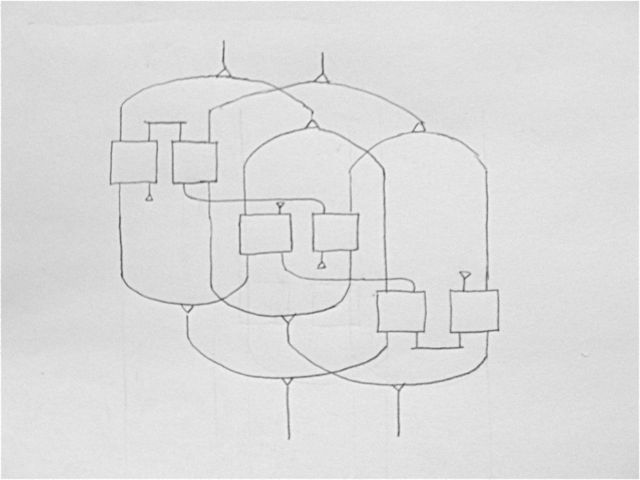
\includegraphics[scale=0.5]{./threeboxes.png}
\end{center}

\end{proof}



% \iflmcs\else\let\oldurl\url\renewcommand{\url}[1]{\hfill\break\oldurl{#1}}\fi
%
% \bibliographystyle{alpha}
% \bibliography{di-biblio}

\end{document}